\scanpage{144}
\figure{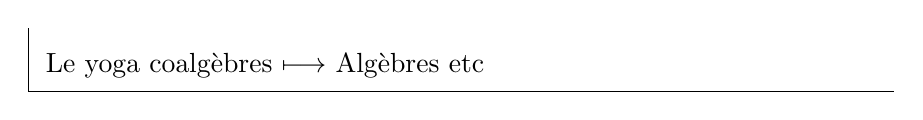
\begin{tikzpicture}\node[anchor=south west] at (0.1,0.05) {Le yoga coalgèbres $\longmapsto$ Algèbres \unsure{etc}};\draw (0,0.8)--(0,0)--(11,0);\end{tikzpicture}}

$\unsure{k}$ anneau, on travaille dans le topos $\widehat C$, où $C_k$ est la catégorie des $k$-algèbres. Le foncteur oubli
\[
C_k\longrightarrow\mathrm{Ens}\qquad A\longmapsto A
\]
est un \deleted{\unsure{faisceau|foncteur} vers les Algèbres}\inserted{objet de $\widehat C_k$ muni d'une structure} de $k$-Algèbre, appelé $O_k$. Si $M$ est un $k$-module, $V(M)$ (\unsure{ou} $V_k(M)$ au besoin) est le \deleted{\unsure{faisceau|foncteur}} $O_k$-Module
\[
V(M)_{\deleted{\unsure{k}}}(\unsure{A})=\operatorname{Hom}_{k\text{-mod}}(M,A)=\operatorname{Hom}_{A\text{-mod}}(M_A,A)
\]
$V(M)$ dépend fonctoriellement de $M$, de façon contravariante, et on voit que $V$ est un foncteur \uline{pl. fd.} des $k$-modules vers les $O_k$-Modules
\[
\operatorname{Hom}_k(M,N)\xrightarrow{\sim}\operatorname{Hom}_{O_k}(V(N),V(M))
\]
\inserted{comme $V(\unsure{N|M})$ est repr. par $\operatorname{Sym}^*(N)$,} De façon générale, un morphisme dans $\widehat C_k$
\[
V(N)\longrightarrow\deleted{V(M)=\operatorname{Spec}(B)}F\qquad(\text{si }F\in\mathrm{ob}\widehat C_k)
\]
\deleted{\unsure{et}} correspond à un \deleted{hom dans $C_k$} élément de $F(\deleted{\unsure{B}}\operatorname{Sym}^*(N))$
\[
\operatorname{Hom}_{\widehat C_k}(V(N),F)\simeq F(\operatorname{Sym}^*(N))
\]
en particulier si $F=\operatorname{Spec} B$
\[
\operatorname{Hom}_{\widehat C_k}(V(N),\operatorname{Spec}B)\simeq
\operatorname{Hom}_{k\text{-alg}}(B,\operatorname{Sym}^*(N))
\]
et faisant $B=\operatorname{Sym}^*(M)$ il vient
\[
\operatorname{Hom}_{\widehat C_k}(V(N),V(M))\simeq
\operatorname{Hom}_{k\text{-mod}}(M,\operatorname{Sym}^*N)
\]
Soit
\[
u^*:V(N)\mathbin{\text{---}}V(M)
\]
correspondant à
\[
u:M\longrightarrow\operatorname{Sym}^*(N).
\]
On \unsure{convient|constate} que
\[
\deleted{\unsure{\lambda^2\longmapsto u(\lambda)}}
\qquad u(m)=\sum u_i(m)\qquad u_i(m)\in\operatorname{Sym}^i(N)
\]
(la famille des \deleted{$\unsure{u_i:M}$} \deleted{\unsure{est} ``loc. finie''}
\[
u_i:M\mathbin{\text{---}}\operatorname{Sym}^i(N)
\]
``loc. finie''), alors on a pour $\lambda\in\unsure{O_k}(A)=A$
\margin{143}
